%%% LaTeX Template
%%% This template is made for project reports
%%%	You may adjust it to your own needs/purposes
%%%
%%% Copyright: http://www.howtotex.com/
%%% Date: March 2011

%%% Preamble
\documentclass[paper=a4, fontsize=12pt]{scrartcl}
\usepackage[T1]{fontenc}
\usepackage{fourier}

\usepackage[utf8]{inputenc}
\usepackage[ngerman]{babel}											
\usepackage[protrusion=true,expansion=true]{microtype}			
\usepackage{amsmath,amsfonts,amsthm}	
\usepackage{IHA_listing}	
\setupListingCpp				
\usepackage[pdftex]{graphicx}													
\usepackage{url}
\usepackage{todonotes}


%%% Custom sectioning (sectsty package)
%\usepackage{sectsty}												
%\allsectionsfont{\centering \normalfont\scshape}	


%%% Custom headers/footers (fancyhdr package)
\usepackage{fancyhdr}
\pagestyle{fancyplain}
\fancyhead{}														% No page header
\fancyfoot[L]{\small Limiter auf dem XMOS DSP}		% You may remove/edit this line 
\fancyfoot[C]{}													% Empty
\fancyfoot[R]{\thepage}									% Pagenumbering
\renewcommand{\headrulewidth}{0pt}			% Remove header underlines
\renewcommand{\footrulewidth}{0pt}				% Remove footer underlines
\setlength{\headheight}{13.6pt}


%%% Equation and float numbering
\numberwithin{equation}{section}		% Equationnumbering: section.eq#
\numberwithin{figure}{section}			% Figurenumbering: section.fig#
\numberwithin{table}{section}				% Tablenumbering: section.tab#

\usepackage[
backend=biber,
style=alphabetic,
sorting=ynt
]{biblatex}
\addbibresource{dsp_refs.bib}

%%% Maketitle metadata
\newcommand{\horrule}[1]{\rule{\linewidth}{#1}} 	% Horizontal rule

\title{
		%\vspace{-1in} 	
		\usefont{OT1}{bch}{b}{n}
		\normalfont \normalsize \textsc{Jadehochschule Oldenburg} \\ [25pt]
		\horrule{0.5pt} \\[0.4cm]
		\huge Look-Ahead Limiter auf einem XMOS Board \\
		\horrule{2pt} \\[0.5cm]
}
\author{
		\normalfont 								\normalsize
        Stephanus Volke\\[-3pt]		\normalsize
        \today
}
\date{}


%%% Begin document
\begin{document}
\maketitle
\newpage
\tableofcontents
\newpage
\section{Einleitung}
Folgender Bericht ist Ergebnis einer Projektarbeit, welche im Sommersemester 2015 an der Jadehochschule Oldenburg im Modul \textit{Digitale Signalprozessoren} unter Leitung von Dr. Uwe Simmer entstand. Inhaltlich beschäftigte sich diese mit der Weiterentwicklung eines im vorhergehenden Semester begonnen, ähnlichen Projektes, welches die Implementierung eines Audio Lookahead Limiters auf einem DSP. Aus diesem Grund soll in diesem Bericht nicht nochmals auf die theoretischen Grundlagen eines Limiters sowie Besonderheiten der Programmierung von digitalen Signalprozessoren in Festkommaarithmetik eingegangen werden. Für Informationen dazu sei auf den entsprechenden Bericht verwiesen \cite{VS15}.


\section{Projektvoraussetzungen}

Dieser Abschnitt befasst sich mit Rahmenbedingungen und Voraussetzungen, welche vor Beginn des Projektes gegeben waren, wobei in Soft- und Hardwaregegebenheiten unterschieden werden soll.

\subsection{Softwarevoraussetzungen}
Als Codebasis stand die in einem vorangegangenen Projekt, ebenfalls von Volke in Zusammenarbeit mit Schreiber erarbeitete Implementierung eines Limiteralgorithmus zur Verfügung \cite{CR00}. Grundlage desselbigen ist die bei Internetrecherche gefundene Realisierungsidee eines nicht weiter identifizierbaren Christians, welche die Besonderheit aufweist, die notwendige Gainregelung in der Attackphase komplett mittels FIR-Filter zu steuern. Das wiederum hat den großen Vorteil, dass der gewählte Schwellenwert wirklich punktgenau erreicht wird und das Ausgangssignal keinesfalls Samples enthält, welche diesen im Pegel überschreiten. Zur Veranschaulichung ist in Abbildung \ref{fig:old_limiter_bsb} der strukturelle Aufbau des Algorithmus dargestellt.


Als frei wählbare Parameter stehen in der Implementierung von Volke und Schreiber der Threshold sowie die jeweiligen Zeiten für Attack- Hold- und Releasphase zur Verfügung. Die Umsetzung erfolge dabei so, dass der Limiter als \textit{loudness maximizer} arbeitet, also die Differenz zwischen Threshold und Vollaussteuerung automatisch mit dem limitierten Signal verrechnet, wodurch ein Ausgangssignal maximaler Lautstärke entsteht.


\subsection{Hardwarevoraussetzungen}
Während die vorliegende Version des Limiters auf dem Blackfin BF533 entwickelt wurde, war es unter anderem Ziel dieses Projektes, die Portierung auf eine andere Hardware Plattform vorzunehmen. Besonders vielversprechend erwies sich dabei das Entwicklungsboard \textit{StartKit} der britischen Firma XMOS. Die Gründe dafür sollen im folgenden Abschnitt erläutert werden.

\section{Vergleich der Hardwarearchitekturen}
Das Entwicklungsboard Blackfin BF-533 von \textit{Analog Devices} hat in den Lehrveranstaltungen im Bereich digitaler Signalprozessoren an der Jadehochschule Oldenburg trotz seines relativ hohen Preises von ca. 450~\$ in den vergangenen Jahren eine dominierende Rolle eingenommen. Ausreichende Performace und eine hohe Zuverlässigkeit sowie die an \textit{Visual Studio} angelehnte und somit vertraute Entwicklungsumgebung \textit{Visual DSP++} sind sicherlich Gründe dieses hohen Stellenwertes. Allerdings drängen seit einigen Jahren auch andere Hersteller mit vielversprechenden Produkten auf den Markt der Signalprozessoren und bieten dabei im Gegensatz zu \textit{Analog Devices} häufig einen großen Vorteil - Entwicklunsgboards zu Preisen, die auch für Studierende erschwinglich sind.
Eine solche Alternative stellt beispielsweise das in diesem Projekt verwendete \textit{StartKit} von XMOS dar, ein Entwicklungsboard mit Multicoreprozessor und sehr flexiblen Einsatzmöglichkeiten, welches lediglich ca. 15 \$ kostet. Tabelle \ref{tab:dps-vergleich} stellt die wesentlichen technischen Eigenschaften des Prozessoren \textit{ADI Blackfin BF533} und \textit{XMOS XS1-A8-64-DEV} gegenüber.
\begin{table}[h!]
\centering
\caption{Vergleich der Prozessorspezifikationen von Blackfin BF533 \cite{TechBF} und XMOS StartKit \cite{TechXMOS}}
\vspace{0.2cm}
  \begin{tabular}{l|cc}
    & ADI Blackfin BF533 & XMOS XS1-A8-64-DEV \\
    \hline
    Architektur 	& DSP 								& RISC + DSP \\
    Kerne 			& 1 									& 8 \\
    Taktfrequenz	& 600 MHz							& 62.5~MHz pro Kern \\
    Multiplizierer 	& 16 Bit fixed						& 32 Bit fixed \\
    Speicher		& 64 kB Speicher + 64 kB Programm 	& 64 kB Speicher + Programm \\
  \end{tabular}
      \label{tab:dps-vergleich}
  \end{table}
  
Tabelle \ref{tab:dps-vergleich} kann entnommen werden, dass es sich bei dem XMOS XS1-A8-64-DEV streng genommen um keinen echten DSP handelt, da er intern nach dem RISC (Reduced Instruction Set Computer) arbeitet. Er besitzt jedoch spezielle Instruktionen um bestimmte Operationen ähnlich effizient wie ein DSP zu verarbeiten.
Von besonderer Bedeutung ist allerdings die Tatsache, dass es sich bei dem Prozessor von XMOS um einen echten multicore Prozessor mit acht logischen Kernen handelt. Diese werden jeweils nacheinander in dezidierten Zeitabschnitten aufgerufen, so dass ein vollkommen deterministischer und vorhersagbarer Programmablauf erreicht wird, der vollständig parallelisierbar ist.
Bedingt durch diese Architektur weist auch die Herangehensweise an die Verarbeitung von Audiodaten einige Besonderheiten im Vergleich zu anderen DSP's und auch dem BF533 auf. Während die Schnittstellen und notwendigen Protokolle zum Einlesen, Verarbeiten und Ausgeben von Audiodaten auf dem Blackfin DSP in Hardware implementiert sind, und somit die gewünschte Aufgabe des Prozessors das erforderliche Hardwaredesign maßgeblich mit beeinflusst, werden all diese Dinge auf dem XMOS Prozessor von Softwarekomponenten übernommen. Zusätzliche Flexibilität wird darüber hinaus durch die Möglichkeit geboten, sogenannte \textit{Slices} an das \textit{XMOS StartKit} anzubringen, welche die für eine bestimmte Aufgabe erforderliche Hardware Komponenten enthalten. Abbildung \ref{fig:audioKit} zeigt beispielsweise die in diesem Projekt verwendete Kombination von \textit{XMOS StartKit} und \textit{Audio Slice}.

\begin{figure}[htb]
  \centering
  \label{fig:audioKit}
  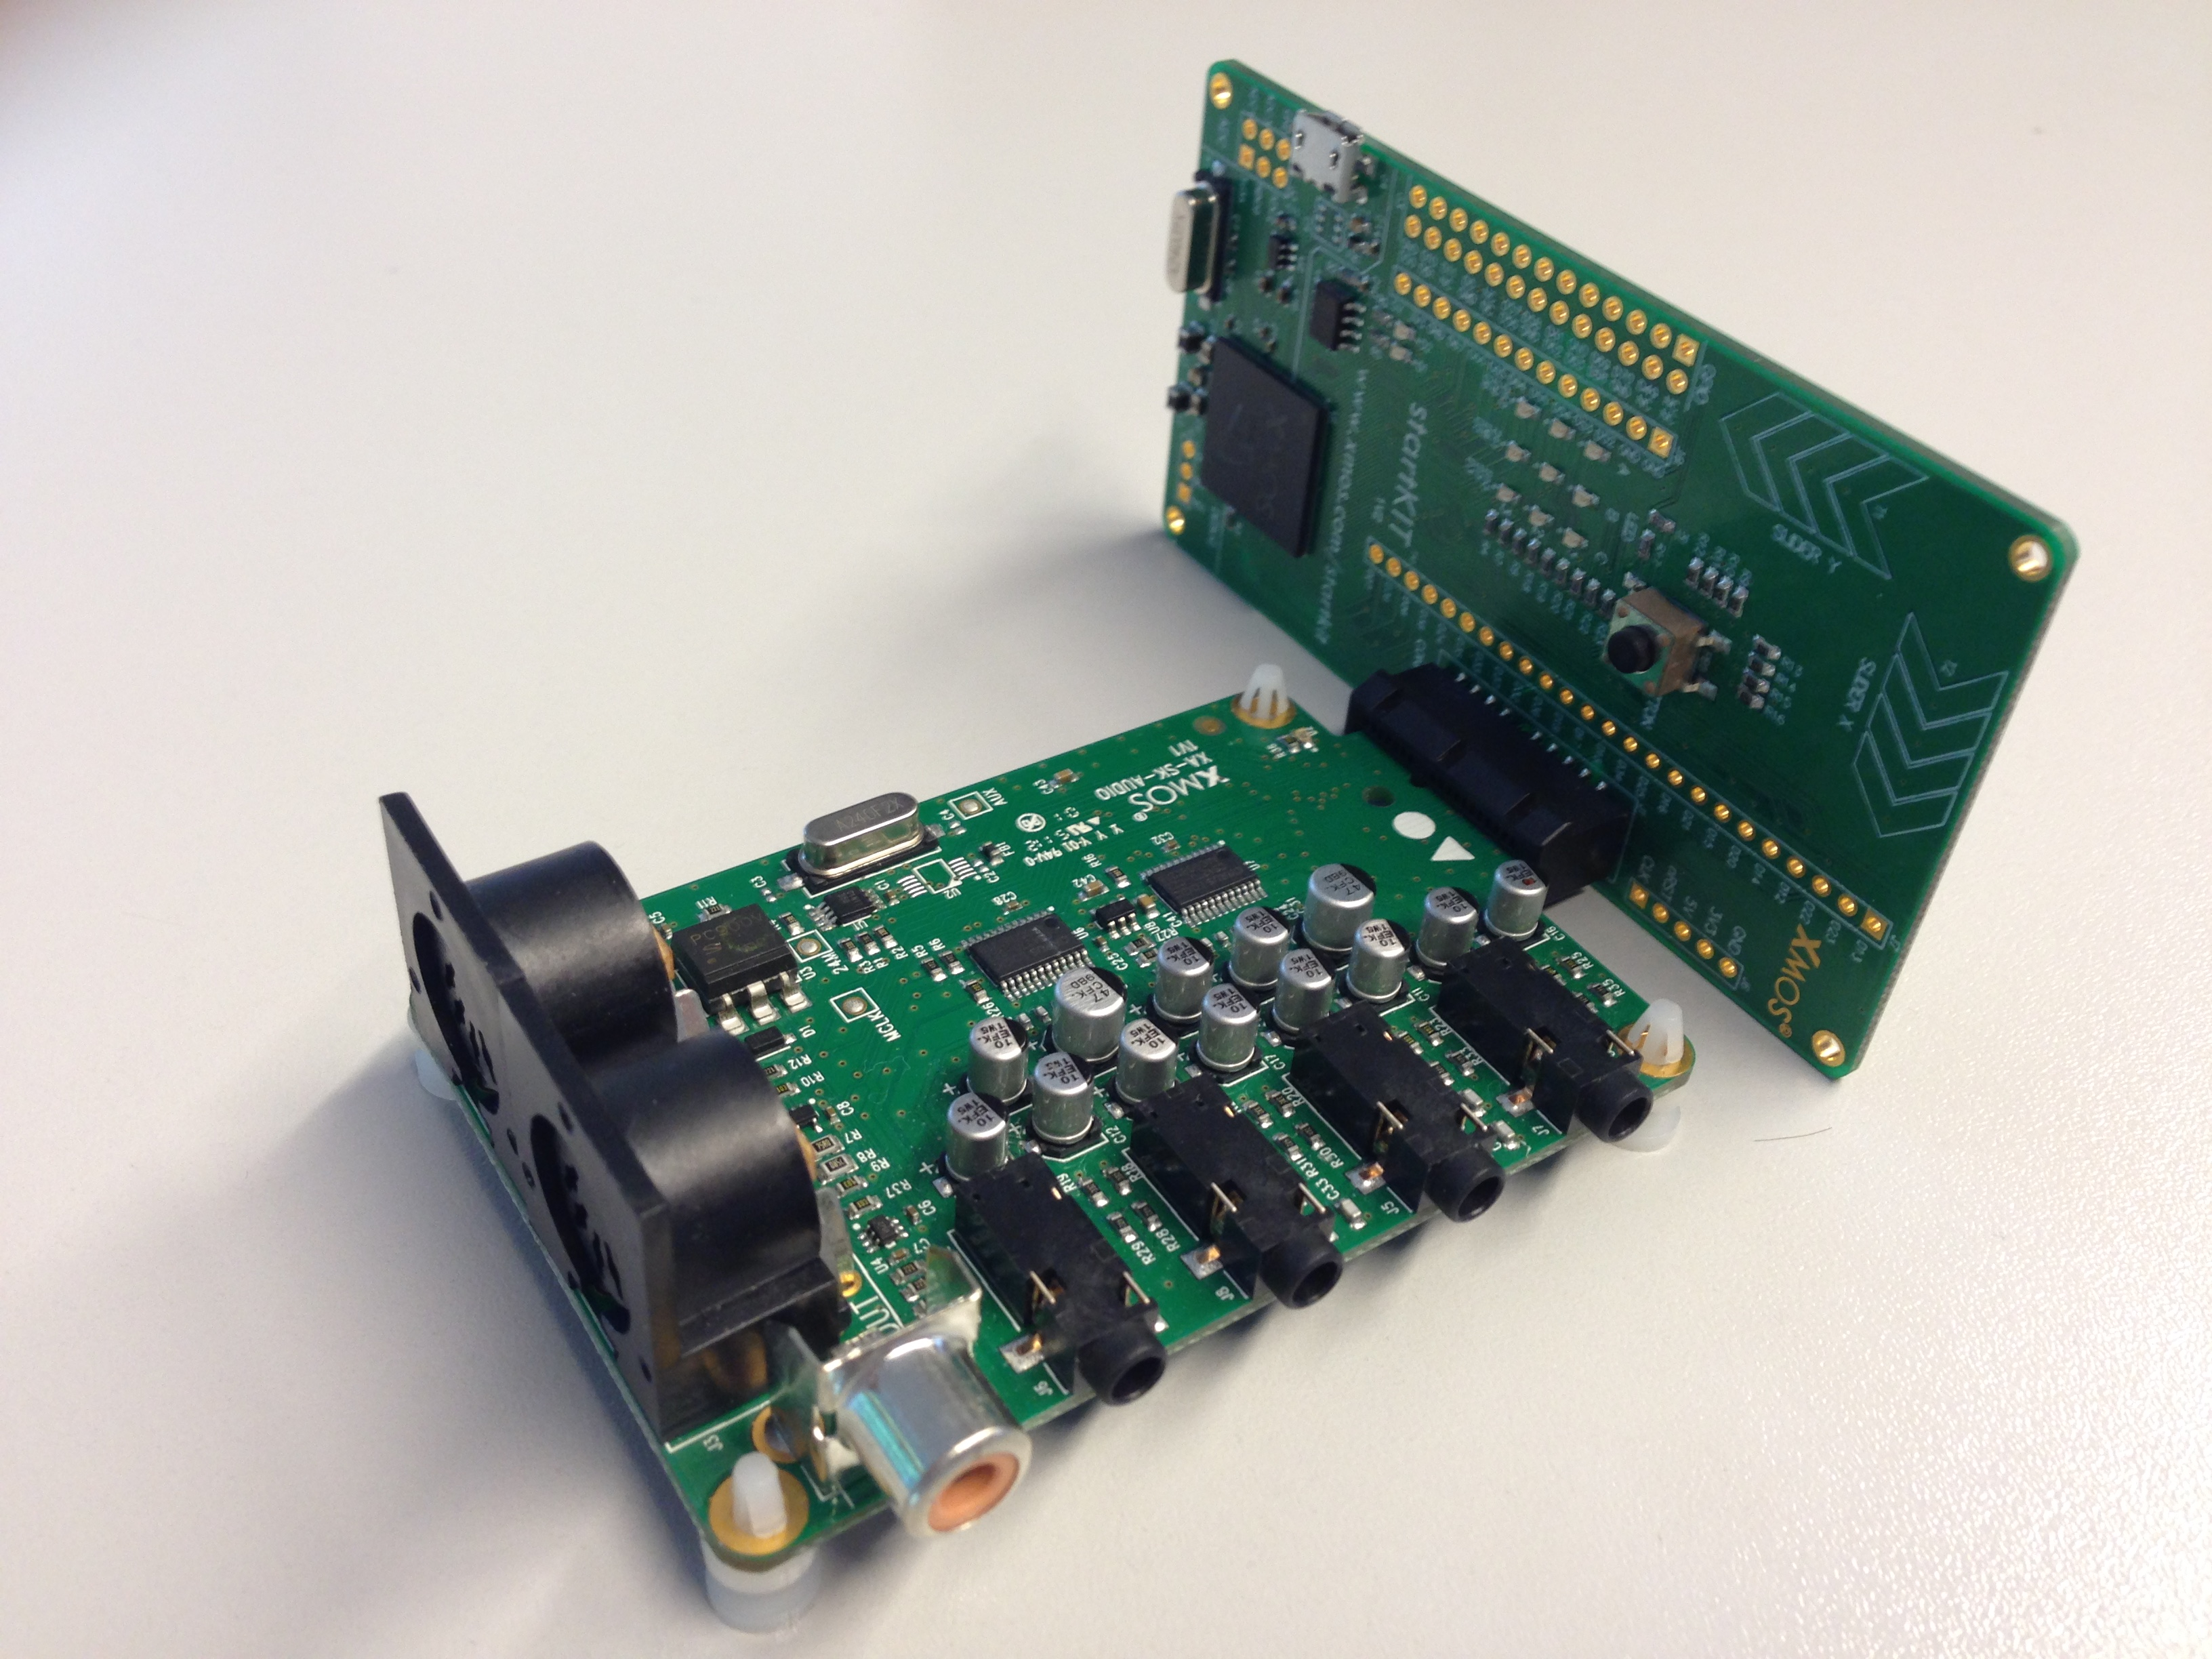
\includegraphics[width=0.8\textwidth]{graphics/IMG_1119}
  \caption{Kombination aus \textit{XMOS StartKit} und \textit{XMOS Audio Slice}}
\end{figure}
 
 
Das \textit{XMOS Audio Slice} stellt dabei folgende Schnittstellen zur Verfügung:

\begin{itemize}
	\item 4 analoge Eingangskanäle via 3.5mm Klinkenbuchse
	\item 4 analoge Ausgangskanäle via 3.5mm Klinkenbuchse
	\item MIDI input/output
	\item SPDIF Ausgang via Coaxialbuchse
\end{itemize}

Zusätzlich sind in der Slicecard die Digital/Analog Konverter sowie die notwendigen Clocks integriert.

\subsection{Gegenüberstellung der Arbeitsweise}
Um die grundsätzliche Vorgehensweise bei der Bearbeitung von Audiodaten auf dem \textit{XMOS StartKit} zu erläutern soll wiederum eine Gegenüberstellung mit dem \textit{Blackfin BF533} vorgenommen werden.\\
Der \textit{BF533} sowie die meisten anderen DSP's arbeiten bei der Kommunikation mit periphären Schnitstellen nach dem Prinzip der sogenannten \textit{Interrupts}. Das bedeutet, dass der Hauptprozess des Programms in einer Endlosschleife läuft und von verschiedenen entweder ereignisorientierten oder zeitbasierten Ereignissen unterbrochen werden kann. Tritt ein solches Ereignis auf, wird eine sogenannte \textit{Service Interrupt Routine (SIR)} aufgerufen, welche die dem Ereignis zugehörige Anweisungsfolge ausführt. Im Falle der Audioverarbeitung auf dem \textit{BF 533} wird ein solcher Interrupt beispielsweise immer dann ausgelöst, wenn der Inputbuffer der Audioschnittstelle voll ist, also ein neuer Block Audiodaten zur Verfügung steht. Das in Endlosschleife laufende Hauptprogramm wird verlassen, in die ISR gesprungen und dort der Code zur Verarbeitung der Audiodaten sowie Freigabe des Inputbuffers und Schreiben des Outputbuffers ausgeführt. Nach Beenden der Anweisungen erfolgt der Rücksprung in das Hauptprogramm bis zum Auftreten des nächsten Interrupts.\\

Demgegenüber steht die Arbeitsweise des \textit{XMOS} Prozessors. Hierbei geschieht die Verarbeitung von periphär gelieferten Daten nicht über ISR's, sondern wird mittels der Parallelisierung umgangen. Die erforderlichen Aufgaben werden auf die verschiedenen Kerne des Prozessors verteilt. So erhält beispielsweise im konkreten Anwendungsfall ein Kern die Aufgabe permanent die Kommunikation zwischen Schnittstelle und Verarbeitungseinheit mittels des i2s Protokolls aufrecht zu halten. Dieses wird, wie viele andere Protokolle auch, von \textit{XMOS} als Softwaremodul bereitgestellt und kann so einfach in eigne Anwendungen integriert werden. Auf diese Weise eingelesene Daten werden an einen weiteren Prozess auf einem anderen Kern weitergeleitet, der quasi parallel die Verarbeitung ausführt.
Da in C keine Sprachkonstrukte für Parallelisierung existieren, kommt auf den Multicoreprozessoren von \textit{XMOS} eine von XMOS entwickelte Erweiterung der Sprache zum Einsatz, in welcher die Syntax von C um Elemente zur Parallelisierung ergänz wurde.

\subsection{Weitere Vorteile des XMOS StartKits}

Das Evaluationsboard \textit{XMOS StartKit} bietet gegenüber dem Blackfin Board noch einige weitere Vorteile. So steht die umfangreiche, auf Eclipse basierende Entwicklungsumgebung \textit{xtimecomposer} kostenlos und für alle gängigen Betriebssysteme (Windows, OS X, Linux) zur Verfügung, während \textit{VisualDSP++} nur für Windows und in Verbindung mit erheblichen Lizensgebühren erhältlich ist.\\

Weiterhin ist das \textit{XMOS StartKit} sehr viel flexibler einsetzbar als der \textit{Blackfin}. Durch seine Erweiterbarkeit durch Slicecards, welche in der Regel nicht teurer als 100 \$ sind (das Audio Slice kostet beispielweise ca. 40 \$), lassen sich unter weitaus geringerem Kostenaufwand vielfältigere Projekte realisieren als bei Verwendung des \textit{Blackfins}.

Eine Besonderheit stellt auch die in \textit{xtimecomposer} integrierte Möglichkeit dar, Daten in Echtzeit zu visualisieren. Dazu steht das sogenannte \textit{xSCOPE} zur Verfügung. In Abbildung \ref{fig:xscope} ist eine beispielhafte Darstellung dieses nützlichen Tools zu sehen, wobei anzumerken ist, dass sich sowohl die Einrichtung als auch Bedienung dieses Werkzeugs immer wieder als kompliziert erweist. Beispielsweise lassen sich die Achseneinteilungen der Darstellung nur sehr umständlich ändern, so dass es mitunter sehr lange dauert, bis der gewünschte Ausschnitt gefunden wird. Die fehlende Möglichkeit diese Einstellungen zu speichern birgt zusätzliches Frustrationpotenzial.

\begin{figure}[htb]
  \centering
  \label{fig:xscope}
  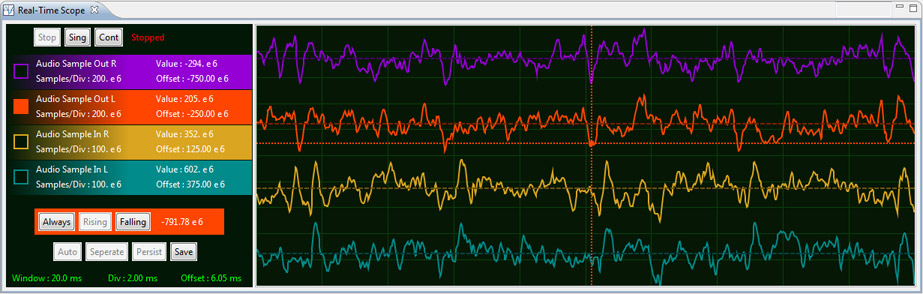
\includegraphics[width=01.0\textwidth]{graphics/xscope.jpg}
  \caption{Beispielhafte Verwendung des in \textit{xtimecomposer} integrierten Echtzeitvisualisierungstools \textit{xSCOPE}}
\end{figure}

Trotz der vielen Vorteile soll an dieser Stelle auch Erwähnung finden, dass der Entwicklungsprozess durch nicht reproduzierbare, willkürlich auftretende und schlecht beschriebene Fehler in der Kommunikation zwischen Entwicklungssoft- und hardware immer wieder erheblich gestört und verzögert wurde. Diese Einschränkung muss unter Berücksichtigung des Kostenvorteiles wohl aber in Kauf genommen werden.

\section{Erweiterungen des Codes}
In den folgenden Abschnitten soll werden die Änderungen und Erweiterungen beschrieben, welche an der bestehenden Codebasis vorgenommen wurden. 

\subsection{Dynamisierung}
Bevor mit der Erweiterung der Funktionalität begonnen wurde, stand die Modifizierung des bestehenden Codes von einer auf Funktionen und modulglobalen Variablen basierenden Implementierung hin zu einer Klassenarchitektur um den Limiter als Einheit aus Variablen und Funktionen besser zu kapseln. Codelisting \ref{lst:class}

\begin{lstlisting}[language=C++, caption={Klassenstruktur der Limiterklasse},label=lst:class,]
class Limiter
{
 public:
  Limiter(float fs, float t_att, float t_hold, float t_rel);
  ~Limiter();
  gains process_sample(int32_t input_sample[], int32_t output_sample[]);
  int32_t getThreshold(void);
  void setThreshold(float newThresh);

 private:
  float   fs;
  float   tAtt;
  float   tHold;
  float   tRel;
  int32_t fixedFS;
  gains return_gains;

  int32_t attBufferLen;
  // weitere state und helper variablen..
  }

\end{lstlisting}

Bei dem Typ \texttt{gains} handelt es sich um eine Struct welches dazu benutzt werden kann, mehrere interessierende Größen zurück zu geben um sie beispielsweise zu plotten. Nach der Initialisierung mittels des Konstruktors, stehen die zwei Methoden \texttt{set/getThreshold} zur Verfügung, mit denen der gewünschte Schwellenwert angepasst bzw. ausgelesen werden kann. Außerdem existiert die Methode \texttt{process\_Sample}, welche ein Eingangssample übergeben bekommt und ein bearbeitetes Ausgangssample zurück liefert.

\subsection{variable Releasezeit}
Limiter mit festen Attack- und Releasezeiten reagieren auf verschiedene Eingangssignale immer gleich. Sobald die Aussteuerung eines Samples den Schwellenwert übersteigt, wird die Attackphase eingeleitet und die Gesamtverstärkung in dieser Zeit entsprechen reduziert, wobei die gewünschte Zielverstärkung innerhalb dieses Zeitfensters erreicht wird. In der eventuell anschließenden Holdphase wird der entsprechende Gain für eine vorher definierte Zeit konstant gehalten um zu schnelle Gainschwankungen, die sich hörbar auf den Klang auswirken könnten, zu vermeiden. Treten innerhlab dieser Holdphase keine weiteren Gainreduzierungen auf, setzt schließlich die Realeasephase ein, in welcher der Gain langsam auf seinen Ausgangswert zurückgeführt wird.

Dieses statische Vorgehen funktioniert für viele Anwendungsfälle gut, birgt aber auch Potenzial für Verbesserungen hinsichtlich der Gainsteuerung. Liegt beispielsweise ein Signal vor, welches im Mittel eine sehr leise Dynamik besitzt und nur an wenigen, markanten Punkten äußerst kurze Signalkomponenten mit lautem Pegel hinzukommen (bspw. Basedrumschläge auf Besenteppich beim Schlagzeug), so führt jeder einzelne Schlag bei ausreichender zeitlicher Trennung zu einem kompletten Durchlauf der eben beschriebenen drei Phasen. Für derartige Fälle lohnt sich die Implementierung eines Algorithmus, der die Fähigkeit besitzt, die Releasezeit an das vorliegende Signal anzupassen.


\subsubsection{Theoretische Grundlagen}
Um laute, kurze Signalanteile in einem ansonsten leisen Signal zu detektieren, bietet sich der sogenannte \textit{Crestfaktor}, welcher für eine gegeben Größe $X$ folgendermaßen definiert ist:

\begin{equation}
\label{eq:crest}
	X_{Crest} = \frac{|X|_{max}}{X_{eff}}
\end{equation}
Als das Verhältnis von Maximalwert und Effektivwert eines Zeitfensters, bietet der Crestfaktor somit eine gute Möglichkeit die genannte Problematik zu quantifizieren. Ein hoher Wert signalisiert ein im Kontext betrachtet auffällig lautes Ereignis, während ein kleiner Wert für eine wenig sprunghafte Dynamik spricht.

\subsubsection{Umsetzung}
Die Anwendung des Crestfaktors als Parameter einer variablen Realeasezeit wurde in Anlehnung an ein Paper von Giannoulis, Massberg und Reiss realisiert.\cite{giannoulis2013parameter}
Zur Berechnung werden zwei zusätzliche Detektoren implementiert, welche nach Gleichungen \ref{eq:peak} und \ref{eq:rms} den aktuellen Peak- bzw. RMS-Wert berechnen. 

\begin{equation}
\label{eq:peak}
	y^2_{Peak}[n] = \text{max}(x^2[n], \alpha y^2_{Peak}[n-1]+(1-\alpha)x^2[n])
\end{equation}
\begin{equation}
	y^2_{RMS}[n] = \alpha y^2_{RMS}[n-1] + (1-\alpha)x^2[n]
\end{equation}
Der notwendige Faktor $\alpha$ ist wie folgt definiert: $$\alpha = e^{\frac{-1}{\tau f_s}} \hspace{0.5cm} \text{mit} \hspace{0.5cm} \tau = 80~\text{ms}, f_s = \text{sampling rate}.$$
Durch die Wahl des identischen $\alpha$ sowohl für Peak- als auch RMS-Detektor ist sicher gestellt, dass der Output des Peakdetektors niemals kleiner als der des RMS-Detektors ist.
Der Crestfaktor würde sich nun nach Gleichung \ref{eq:crest} aus $$y_{Crest}[n] = \sqrt{\frac{y^2_{Peak}[n]}{y^2_{RMS}[n]}}$$ berechnen. Allerdings wird in Anlehnung an Gleichung (8) aus \cite{giannoulis2013parameter} die Zeitkonstante für die adaptive Releasezeit $\tau_R[n]$ folgendermaßen bestimmt
\begin{equation}
\label{eq:tauR}
	\tau_R[n] = 2\tau_{R~\text{max}}/y^2_{Crest}[n] - \tau_{A},
\end{equation}
wobei $\tau_{R~\text{Max}}$ die maximale Releasezeit und $\tau_A$ die festgesetzte Attackzeit angeben.
Um eine in fixed point Arithmetik \textit{teure} Division einzusparen wird die Bestimmung des notwendigen $\tau_R[n]$ unter Verwendung von Gleichungen \ref{eq:crest} und \ref{eq:tauR} folgendermaßen realisiert

\begin{equation}
	\tau_R[n] = 2\tau_{R~\text{max}} \cdot \frac{1}{y^2_{Crest}[n]},
\end{equation} 
was dazu führt, anstelle von Gleichung \ref{eq:crest} direkt dessen Kehrwert
$$\frac{1}{y^2_{Crest}[n]} = \frac{y^2_{RMS}[n]}{y^2_{Peak}[n]}$$
zu berechnen.

Als letzten Schritt muss nun aus der nun adaptiven Zeitkonstante $\tau_R[n]$ der entsprechende Koeffizient für das IIR-Filter der Releasephase berechnet werden, was mittels folgender Berechnungsvorschrift geschieht:
$$1-\alpha = \frac{1}{f_s*\tau_R[n]}$$

In Listing \ref{lst:crest-code} sind die eben beschriebene mathematischen Zusammenhänge in der Codeimplementierung umgesetzt

\begin{lstlisting}[language=C++, label=lst:crest-code, caption={Darstellung des für die Crestfaktorberechnug relevanten Codes}]
// necessary variables
alpha = float_to_fixed32(exp(-1/(0.2*fs)),31);

// Peak detector
x2n = max(abs(output_sample[0]), abs(output_sample[1]));
x2n = ((int64_t)x2n*x2n) >> 31;
Peak = max(x2n,(((int64_t)alpha*Peak) >> 31) + 
	   (((int64_t)(0x7fffffff-alpha)*x2n) >> 31));
	   
// RMS detector
Rms = (((int64_t)alpha*Rms) >> 31) + (((int64_t)(0x7fffffff-alpha)*x2n) >> 31);

// calc inverted crest factor
crest2Inv = udiv32(Rms,Peak);

// calc time constant
tauRel = tRelMax << 1; // 1s * 2 = 2s
tauRel = (((int64_t) tauRel * crest2Inv) >> 16) - tAtt;

// calc coefficents
crest_bRel = udiv32(fixedFS, tauRel);
crest_aRel = 0x7fffffff-crest_bRel;

// Release mittels IIR Filter mit Crest
if (crest_gain > crest_oldGain)
{
    temp64  = (int64_t) crest_aRel * crest_oldGain;
    temp64 += (int64_t) crest_bRel * crest_gain;
    crest_gain = min(crest_gain, (int32_t) (temp64 >> 31));
}
crest_oldGain = crest_gain;	
\end{lstlisting}

Um eine bessere Evaluation durchführen zu können wird zusätzlich auch jeweils der Gain mit fester Releasezeit berechnet und steht somit  als optionaler Rückgabewert zur Verfügung. 

\section{Evaluation}

Für eine umfangreiche Evaluation fehlte in Rahmen des Modules \textit{Digitale Signalprozessoren} die Zeit. Wünschenswert wäre insbesondere eine sich auf Hörtests stützende Bewertung des mittels adaptiver Releasephase erweiterten Limiteralgorithmus im Vergleich zur Standardvariante. Der subjektive Höreindruck der am Modul beteiligten Personen war der übereinstimmenden Meinung, dass besonders Signale mit großen Dynamiksprüngen tendenziell etwas lauter wahrgenommen werden. Diese Beobachtung erscheint logisch, da die Gainregelung in diesem Falle sehr schnell erfolgt und so fast immer der maximal mögliche Gain auftritt.

Auf Grund der fehlenden subjektiven Bewertung soll an dieser Stelle ein kleiner objektiver Blick auf die Auswirkung des vorgestellten Algorithmus geworfen werden. Dazu wurden für verschiedene Signale (Drumset, Gitarre solo, Rockband) vergleichende Grafiken bezüglich des Gainverlaufes mit und ohne adaptiver Releasephase erstellt. Diese sind in den Abbildungen \ref{fig:drums}, \ref{fig:guitar} und \ref{fig:band} zu sehen.

\begin{figure}[h!]
  \centering
  \label{fig:drums}
  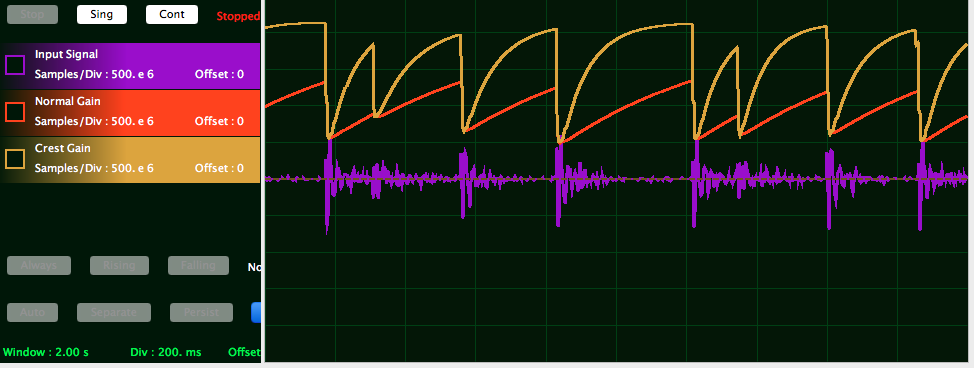
\includegraphics[width=0.9\textwidth]{graphics/drums_gains}
  \caption{Aufgenommenes Schlagzeug.}
\end{figure}

\begin{figure}[h!]
  \centering
  \label{fig:guitar}
  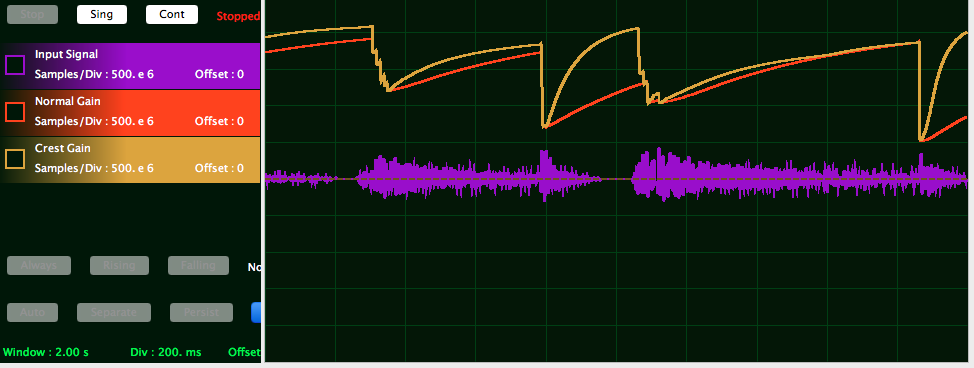
\includegraphics[width=.9\textwidth]{graphics/guitar_gains}
  \caption{Beispielhafte Verwendung des in \textit{xtimecomposer} integrierten Echtzeitvisualisierungstools \textit{xSCOPE}}
\end{figure}

Beide Abbildungen zeigen die Wirkungsweise des Algorithmus sehr gut. Während die rot dargestellte fixe Releasephase immer in gleicher Weise dem Vollaussteuerung entgegenstrebt, variiert das Verhalten der gelben, adaptierten Kurve. 

 

\section{Fazit}




%%% End document

\printbibliography
\end{document}